\documentclass[sigconf]{acmart}
% % Packages
\usepackage{soul}
% \usepackage{cite}
% \usepackage{balance}
% \usepackage{listings}
% \usepackage{amsmath,amssymb,amsfonts}
% \usepackage{algorithmic}
% \usepackage{graphicx}
% \usepackage{textcomp}
% \usepackage{xcolor}
% \usepackage{booktabs}
% \usepackage{enumitem}
% \usepackage{hyperref}
% \usepackage{totpages}
% \usepackage{subcaption}

%% \BibTeX command to typeset BibTeX logo in the docs
\AtBeginDocument{%
  \providecommand\BibTeX{{%
    \normalfont B\kern-0.5em{\scshape i\kern-0.25em b}\kern-0.8em\TeX}}}

\begin{document}

% Specify path to images
\graphicspath{ {./img/} }


%%
%% The "title" command has an optional parameter,
%% allowing the author to define a "short title" to be used in page headers.
\title[Contrast Subgraphs of Brain Networks]{Improvements and Discussion of "Explainable Classification of Brain Networks via Contrast Subgraphs"}

\author{Tengkai Yu}
\email{FIXTHIS@uvic.ca}
\affiliation{%
  \institution{University of Victoria}
  \department{Computer Science}
  \streetaddress{PO Box 1700 STN CSC}
  \city{Victoria}
  \state{British Columbia}
  \country{Canada}
  \postcode{V8W 2Y2}
}

\author{Keanelek Enns}
\email{keanelekenns@uvic.ca}
\affiliation{%
  \institution{University of Victoria}
  \department{Computer Science}
  \streetaddress{PO Box 1700 STN CSC}
  \city{Victoria}
  \state{British Columbia}
  \country{Canada}
  \postcode{V8W 2Y2}
}

\author{Venkatesh Srinivasan}
\email{srinivas@uvic.ca}
\affiliation{%
  \institution{University of Victoria}
  \department{Computer Science}
  \streetaddress{PO Box 1700 STN CSC}
  \city{Victoria}
  \state{British Columbia}
  \country{Canada}
  \postcode{V8W 2Y2}
}

\author{Alex Thomo}
\email{thomo@uvic.ca}
\affiliation{%
  \institution{University of Victoria}
  \department{Computer Science}
  \streetaddress{PO Box 1700 STN CSC}
  \city{Victoria}
  \state{British Columbia}
  \country{Canada}
  \postcode{V8W 2Y2}
}

%%
%% By default, the full list of authors will be used in the page
%% headers. Often, this list is too long, and will overlap
%% other information printed in the page headers. This command allows
%% the author to define a more concise list
%% of authors' names for this purpose.
\renewcommand{\shortauthors}{T. Yu and K. Enns}

%%
%% The abstract is a short summary of the work to be presented in the
%% article.
\begin{abstract}
\hl{TODO}
\end{abstract}

%%
%% The code below is generated by the tool at http://dl.acm.org/ccs.cfm.
%%
\begin{CCSXML}
<ccs2012>
   <concept>
       <concept_id>10002950.10003624.10003633.10010917</concept_id>
       <concept_desc>Mathematics of computing~Graph algorithms</concept_desc>
       <concept_significance>500</concept_significance>
       </concept>
   <concept>
       <concept_id>10010405.10010444.10010446</concept_id>
       <concept_desc>Applied computing~Consumer health</concept_desc>
       <concept_significance>300</concept_significance>
       </concept>
 </ccs2012>
\end{CCSXML}

\ccsdesc[500]{Mathematics of computing~Graph algorithms}
\ccsdesc[300]{Applied computing~Consumer health}

%%
%% Keywords. The author(s) should pick words that accurately describe
%% the work being presented. Separate the keywords with commas.
\keywords{graph analytics, graph algorithms, brain networks, densest subgraph}

\settopmatter{printfolios=true} % for page numbering

%% This command processes the author and affiliation and title
%% information and builds the first part of the formatted document.
\maketitle

\section{Introduction} \label{intro}

Graphs are used to represent a wide variety of complex entities, systems, and relationships.
As their use continues to grow in many areas of research and industry, graph classification, the process of labelling graphs as belonging to certain categories or classes, has become increasingly important \hl{find a citation to back up importance claim}.
One particularly interesting graph classification problem comes in the form of identifying individuals possessing certain neurological disorders by considering graphs that model functional connections in the brain (referred to as brain networks).

There are multiple ways to measure the quality of a graph classification model.
Metrics such as accuracy, precision, and recall are essential for evaluating any classifier \cite{elkan2012}, but recently there has been a trend towards explainability in the world of machine learning and artificial intelligence \cite{hassan2021,linardatos2020}.
This is because industries, governments, and organizations, especially those that deal with critical decision making such as the medical field, are hesitant to adopt prediction models without knowing \emph{how and why} they make decisions, regardless of how accurate these models are reported to be.
Therefore, it is increasingly important to find a balance between classification models that are explainable and simple to understand, while also achieving high accuracy, precision, and recall scores.

Explainability in classifiers is not only about building confidence in the user of the classifier.
Providing insights that may not have been detected through classical methods is another major benefit and may lead to further advancements in research.
These insights are especially helpful to neuroscientists when it comes to studying less understood neurological disorders such as Autism Spectrum Disorder (ASD).

The question at the core of this study is, \emph{"What information in a brain network can be used to discern between individuals with ASD and those typically developed (TD)?"}
Rather than plugging a group of brain networks into a black box classifier and asking it to predict the class of new brain networks, we would like to identify intuitive features of the networks so that we know \emph{why} a given network is being classified the way it is.
Thankfully, others have come before us with a similar goal.

In their paper, "Explainable Classification of Brain Networks via Contrast Subgraphs", Lanciano \emph{et al.} proposed a method for translating brain networks into two dimensional representations with a simple interpretation \cite{lanciano2020}.
This translation of a graph into a vector representation is known as a graph embedding and is fundamental to many graph classification problems \cite{goyal2018}.
The graph embedding employed by Lanciano \emph{et al.} involves the use of contrast subgraphs, which we define in section \ref{emb-technique}.

In this study, we sought to replicate the findings of Lanciano \emph{et al.} as well as discover alternatives or improvements to the methods described in their paper (referred to as the original paper from here on) \cite{lanciano2020}.
We found the quantitative results reported in the original paper were not reproducible, and much of the implementation was unavailable in the given replication package\footnote{The original paper's replication package can be found at \url{https://github.com/tlancian/contrast-subgraph} and was accessed in January 2022.}.
In light of this, we summarize our contributions as follows:

\begin{itemize}
    \item We provide a complete and optimized implementation of the original paper's graph embedding process\footnote{Our replication package can be found at \url{https://github.com/keanelekenns/contrast-subgraph}.}.
    \item We demonstrate various improvements to the original paper's methods such as 
    \begin{itemize}
        \item using a quadratic programming (QP) solver instead of a semidefinite programming (SDP) solver.
        \item optimizing the local search algorithm used.
        \item utilizing the top-k contrast subgraphs, as suggested by the original authors for future work.
    \end{itemize}
    \item We develop an entirely new graph embedding technique named Discriminative Edges (DE) that provides improved accuracy and reduced computational time over the original paper's methods, all while maintaining similar explainability.
    \item We provide code for evaluating the graph classification approaches along with recording specific parameters used and results associated with them.
\end{itemize}

The following section will discuss related works.
Section \ref{problem-statement} will give more context for the problem we are solving, along with a description of the solutions we plan to apply.
The process followed and the results obtained are outlined in section \ref{experiments}, and finally, we end the paper with discussions and conclusions for this study.

\section{Related Work} \label{related-work}

\hl{Are you supposed to mention the paper you are replicating in the related works? Also, to what extent should we mention the papers that Lanciano built off of?}

\hl{Talk about trend towards explainability in AI (xAI). A possible reference is https://doi.org/10.1016/j.inffus.2021.01.008}

Dai and Wang worked on creating explanations that are built into a GNN \cite{dai2021} rather than trying to find an explanation after the GNN had made its classification.
They found their method to be less biased and more computationally efficient when compared to using a post-hoc explainer such as GNN explainer.

Wang \emph{et al.} recently proposed a method, named DHC-E, for embedding graphs in a generalizable way that does not require any hyperparameters \cite{wang2021}. The embedding has a moderate number of dimensions depending on the graph set analyzed and is based on the h-index values of each vertex in the graph. They used principal component analysis to present the graph embeddings in two dimensions.

\hl{Look into https://doi.org/10.1142/S0129183118400077,

https://dl.acm.org/doi/abs/10.1145/3219819.3219980}

\section{Problem Statement} \label{problem-statement}

There are three main components for creating a graph classification model:

\begin{enumerate}
    \item Embedding technique: This is how the complex information of a graph is translated into a simplified representation. This representation often comes in the form of a real valued vector where each value is called a "feature".
    \item Classifier algorithm: This is the method of training the model to discern between (embedded) graphs of each class.
    \item Data: The instances (in this case, brain networks) that the model is trained with.
\end{enumerate}

\textbf{Embedding Technique.}
This paper focuses primarily on developing embedding techniques.
The techniques involve the use of contrast subgraphs and discriminative edges.
We give more thorough discussions of these techniques in the following sections.

\textbf{Classifier Algorithm.}
LinearSVC was chosen from the commonly used scikit-learn python library as a baseline classifier algorithm and was used for all the experiments.
This allows us to fairly compare the embedding techniques used.

\textbf{Data.}
A common group of data sets were used for the experiments.
Data from the Autism Brain Imaging Data Exchange (ABIDE) project \cite{craddock2013} was processed by Lanciano \emph{et al.}.
This processing resulted in groups of undirected, unweighted graphs (brain networks) defined over a common set of 116 vertices.
The vertices of the brain networks correspond to regions of interest (ROIs) in the brain, thus we are studying a special case of graph classification where all considered graphs possess the same set of vertices (i.e. regions of the brain which are, naturally, common to all brains).
The edges of each brain network correspond to functional (as opposed to structural) connections in the brain.
For a more thorough discussion of the data sets used and the processing that was performed by Lanciano \emph{et al.}, please see section 5 of the original paper \cite{lanciano2020}.

\subsection{Embedding Techniques} \label{emb-technique}
When it comes to creating an embedding technique in the context of brain network classification, the question we are asking is, \emph{"How can we translate a brain network into a vector/embedding in such a way that the embedding is intuitive \textbf{and} adequately separates different brain networks according to their classes?"}

The embedding must be intuitive in order for our classification model to be explainable and simple to understand.

The embedding must also separate the different classes of brain networks in order to help the classification algorithm learn the differences between them.
In the case of vector embeddings, this literally means that we want the vectors of each class to be as far apart from each other as they can be.

\textbf{Notation.}
We reuse the notation specified in the original paper and reiterate the important notation here.

Let the $i^{th}$ brain network be represented as an undirected, unweighted graph $G_i = (V, E_i)$, where $V$ is the common vertex set representing the 116 ROIs of the brain as discussed previously (i.e. $|V| = 116$) and $E_i$ is the set of edges belonging to $G_i$ (note: $E_i \subset V \times V$).

Let a \emph{summary graph} corresponding to a set of brain networks $\mathcal{A}$ be a weighted, undirected graph $G^{\mathcal{A}} = (V, w^{\mathcal{A}})$, where $w^{\mathcal{A}}: V \times V \rightarrow \mathbb{R}_+$ is a weight function that assigns a value to each pair of vertices in $V$.
For vertices $u,v \in V$, we define $w^{\mathcal{A}}(u,v)$ to be the fraction of networks in $\mathcal{A}$ that contain the edge $(u,v)$.


\subsubsection{Contrast Subgraph.}
A contrast subgraph is defined as a subset of vertices, that induces a dense subgraph in one graph and a sparse subgraph in another, assuming that the graphs share a common vertex set.
The problem can be simplified to finding a set of vertices that induce a dense subgraph in the difference of the two graphs (in this case, summary graphs of each class).
We echo the problem definition of the original paper.

\emph{Problem 1 (Contrast Subgraph). Given two sets of observation graphs, i.e. the condition group $\mathcal{A} = \{G^{\mathcal{A}}_1, . . . , G^{\mathcal{A}}_{|\mathcal{A}|}\}$ and the control group $\mathcal{B} = \{G^{\mathcal{B}}_1, . . . , G^{\mathcal{B}}_{|\mathcal{B}|}\}$, and corresponding summary graphs $G^{\mathcal{A}} = (V, w^{\mathcal{A}})$ and $G^{\mathcal{B}} = (V, w^{\mathcal{B}})$, we seek to find a subset of vertices $S^* \subseteq V$ that maximizes the contrast subgraph objective}
\begin{align*}
    \delta (S) = \sum_{u,v \in S} \left(w^{\mathcal{A}}(u,v) - w^{\mathcal{B}}(u,v) - \alpha\right)
\end{align*}
\emph{where $\alpha \in \mathbb{R}_+$ is a user-defined parameter.}

The original paper also defines a symmetric variant of the contrast subgraph problem (\emph{Problem 2}) which shares the same definition of \emph{Problem 1}, but with an alternative objective

\begin{align*}
    \sigma (S) = \sum_{u,v \in S} \left(|w^{\mathcal{A}}(u,v) - w^{\mathcal{B}}(u,v)| - \alpha\right)
\end{align*}

The parameter $\alpha$ is used to penalize large contrast subgraphs and to avoid the trivial solution $S^* = V$.
It can be adjusted to vary the proportion of edges that are considered detrimental to the contrast subgraph objective.

Once a contrast subgraph is obtained, it can be used in the following ways to embed a graph.

\textbf{Problem 1.}
The original authors use contrast sugbraph overlap to create two features for each brain network.
Because the problem is asymmetric, two contrast subgraphs are obtained.
One is found using the difference network $G^{TD - ASD}$ (which is the result of subtracting the summary graph of the TD brain networks from the summary graph of the ASD brain networks) and the other is found using $G^{ASD - TD}$.
Each feature corresponds to the number of edges in common between the brain network and the two contrast subgraphs.

\textbf{Problem 2.}
Only one contrast subgraph is obtained with this embedding technique.
The contrast subgraph is used to induce subgraphs in both of the summary graphs (i.e. $G^{TD}$ and $G^{ASD}$) as well as each individual brain network.
The distance from the induced brain network and each summary graph is then used as the two features for this embedding.

\subsubsection{Discriminative Edges.}


\section{Experiments} \label{experiments}

\begin{figure}
    \centering
    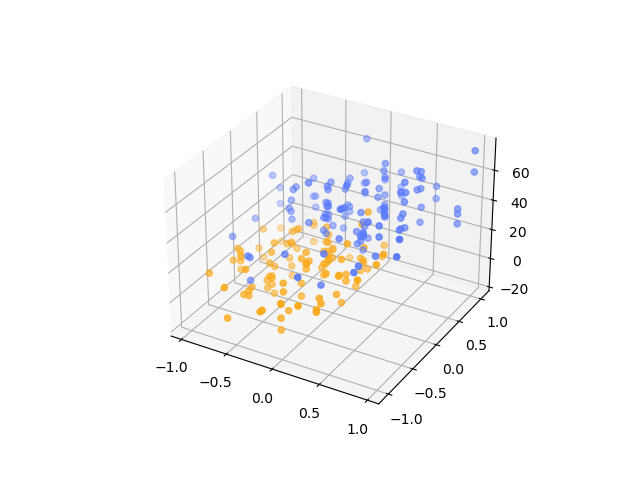
\includegraphics[width=\columnwidth, keepaspectratio=true]{test.png}
    \caption{\hl{This is just a test image, we need to create proper images with proper labels}}
    \label{fig:my_label}
\end{figure}

\section{Limitations and Threats to Validity} \label{limitations}

This study was limited primarily by the data set used.
In many machine learning applications, a large volume of data is needed to adequately train and test new models.
With a small data set, it is difficult to know how generalizable any of the discussed methods are to new brain networks that we wish to classify.
Additionally, the way the data set was created and the individuals that were studied have a large impact on the validity of the classification methods developed.
Elkan gave a helpful discussion of potential pitfalls regarding evaluating classifiers and the way data is gathered \cite{elkan2012}.
In this case, the limitations in data set size and quantity are due to the costly nature of creating such brain networks as individuals need to undergo a series of scans and time series of these scans are used to create the resultant brain network \cite{lanciano2020}.
Furthermore, the ratio of the studied classes is imbalanced when compared to the true ratio of individuals with ASD.

Autism Spectrum Disorder is a very complex disorder with unclear definitions, and it may manifest in various different ways [\hl{perhaps this belongs in the intro when describing why the problem is hard?}].
Above all this, the brain is a highly complex organ that is not fully understood.
The brains of individuals are unique and develop in complex manners.
There may be a plethora of confounding factors that have an effect on the classification of such networks with respect to identifying ASD in individuals.

\section{Discussion} \label{discussion}

Lanciano \emph{et al.} showed that the degrees of each vertex in the studied brain networks did not vary significantly between the two classes \cite{lanciano2020},
yet the contrast subgraphs are defined as a set of vertices, and every edge induced by these vertices is used for classification.
Instead, we should look solely at edges that are important for distinguishing between the classes.

The discriminative edge method considers the most important edges in each class (defined as having the most positive and most negative weights in the difference network) when creating an embedding.
Additionally, it considers the brain network as a whole in its third dimension, which likely captures more interesting information with respect to complex connections in the brain.
However, it does not specifically identify higher order structures in the brain networks that may be leading to the DNN's success.

\section{Conclusion} \label{conclusion}

Future work should attempt to identify higher order structures (such as triangles, k-clusters, or graphlets of varying size and shapes) as a means of embedding.
This could be done by identifying prominent structures in each summary graph (perhaps after thresholding the edge weights), eliminating structures common to both, and counting the number of overlapping structures that a new brain network has in common with each class.
The challenge associated with this technique comes with the computational complexity of enumerating such high order structures.

As discussed in section \ref{limitations}, this study should be replicated on additional data sets to further test its validity.

\bibliographystyle{ACM-Reference-Format}
\bibliography{refs.bib}

\appendix
\section*{APPENDICES}
\section{Artifacts} \label{artifacts}

Project Repository:

\url{https://github.com/keanelekenns/contrast-subgraph}

\end{document}
\endinput